\documentclass[conference]{IEEEtran}
\usepackage[T1]{fontenc}
\usepackage{graphicx,amsmath,amssymb,booktabs,xurl}
\usepackage[hidelinks]{hyperref}
\title{Graph-Attention Traffic Forecasting and Synthetic LWR Signal Control}
\author{\IEEEauthorblockN{Kavya Katal, Rudraksh Sharma, Anshuman Mehta, Vridhi Chaudhary, Bineet Keshari}
\IEEEauthorblockA{Team T072, Section C, Rishihood University\\Deep Learning Project, November 2026}}
\begin{document}
\raggedbottom
\maketitle
\begin{abstract}
We extend independent-sensor machine-learning forecasting with a shared gated recurrent unit (GRU) and a GRU plus graph-attention network (GAT). The study tests whether supplied road-network connectivity adds value under matched chronological evaluation. Training-only normalization, causal histories and masked labels support controlled comparisons. Self-loop, uniform-attention and dropout variants examine component contributions. A validation-selected XGBoost blend tests an optional hybrid. Results remain exploratory because the historical test interval was previously inspected. A separate synthetic LWR cell-transmission experiment compares fixed signals with two local rule-based agents. The simulator is not calibrated to METR-LA; no learned policy, GAT-driven control or real-world benefit is claimed.
\IfFileExists{generated/abstract_results.tex}{ At 60 minutes, graph-model MAE averaged across three seeds is 4.881 mph, compared with 4.931 mph for the self-loop control and 3.874 mph for frozen XGBoost. Neighbour access improves the neural control but does not surpass XGBoost.
}{}
\end{abstract}
\begin{IEEEkeywords}traffic forecasting, METR-LA, GRU, graph attention, ablation\end{IEEEkeywords}

\section{Problem and Literature}
We forecast 12 future speeds from 12 observed five-minute sampling slots per sensor. Headline horizons are 15, 30 and 60 minutes. Traffic varies over time and across connected locations; forecasting can inform later traffic-management studies, but alone does not demonstrate a control benefit. Phase 1 supplied persistence, historical average, Random Forest and XGBoost references. We test whether neighbours help beyond temporal learning.

Cho et al. motivate gated temporal representation \cite{cho}. GAT learns masked neighbourhood aggregation \cite{gat}. DCRNN provides traffic-forecasting context \cite{dcrnn}; our architecture is not its reproduction, and different published protocols prevent direct score rankings. The allocated project title motivates graph forecasting and LWR theory. The real-data experiment concerns speed forecasting. A separate illustrative LWR/control experiment uses synthetic road parameters and arrivals; the two components are not a calibrated predictive-control system.

\section{Data and Preparation}
METR-LA contains 34,272 timestamps and 207 sensors, from March 1 to June 27, 2012, every five minutes. Benchmark units are mph; timezone is unencoded. Zero/NaN readings are missing by convention, not physical proof of an outage. Full-file missingness is 8.11\%; training-fit missingness is 7.13\%. Training EDA covers distributions, daily profiles, missingness, gap lengths, histories and locations.

Each history uses $t-11,\ldots,t$, 55 minutes between endpoints. Fill forward only inside that history; leading gaps use training sensor medians. An entirely unobserved training sensor would use global training mean. Original missingness flags remain; future targets are never filled. Fit global normalization mean/std only on valid training speeds, then restore mph for scoring.

Neural input is $B\times12\times207\times2$: normalized speed and missingness. Both models receive five origin-calendar features (daily/weekly sine-cosine pairs, weekend). Output is $B\times12\times207$. Trees use 38 engineered features, so ML--DL comparisons compare pipelines rather than isolating graph information.

The fit interval ends at the last training target, equal to the first tuning-validation origin; no validation target enters these statistics. Previously observed history may cross split boundaries.

\section{Architecture}
A shared one-layer GRU with 32 hidden units encodes each sensor independently. In compact notation for the installed PyTorch GRU \cite{torchgru}:
\begin{align}
r_t&=\sigma(W_rx_t+U_rh_{t-1}+b_r),\\
u_t&=\sigma(W_ux_t+U_uh_{t-1}+b_u),\\
n_t&=\tanh(W_nx_t+b_n+r_t\odot(U_nh_{t-1}+c_n)),\\
h_t&=(1-u_t)\odot n_t+u_t\odot h_{t-1}.
\end{align}
Here $r_t$ resets candidate memory, $u_t$ controls retention, $\sigma$ is sigmoid and $\odot$ is elementwise multiplication. Each window starts from zero hidden state. The temporal model feeds local embedding and calendar features to a linear 12-output head. The graph model also includes one GAT aggregate (two 16-channel heads).
\begin{figure*}[t]
\centering\small
\begin{tabular}{c@{\quad}c@{\quad}c@{\quad}c@{\quad}c@{\quad}c@{\quad}c}
\shortstack{12 observed slots\\speed + missing flag} & $\rightarrow$ &
\shortstack{Shared GRU\\32 values/sensor} & $\rightarrow$ &
\shortstack{Local + calendar\\linear head} & $\rightarrow$ &
\shortstack{12 corrections\\+ latest filled speed}\\[12pt]
\shortstack{All sensor\\GRU embeddings} & $\rightarrow$ &
\shortstack{Masked GAT\\2 heads $\times$ 16} & $\rightarrow$ &
\shortstack{Local + graph + calendar\\linear head} & $\rightarrow$ &
\shortstack{12 corrections\\+ latest filled speed}
\end{tabular}
\caption{Temporal baseline (top) and graph model (bottom). Heads receive the same five origin-calendar features. Graph aggregation uses only permitted sender nodes; each forecast contains 12 future speeds for each of 207 sensors.}
\label{fig:architecture}
\end{figure*}
For one graph-attention head:
\begin{align}
e_{ij}&=\operatorname{LeakyReLU}(a_r^\top Wz_i+a_s^\top Wz_j),\\
\alpha_{ij}&=\exp(e_{ij})/\sum_{k\in\mathcal N_i}\exp(e_{ik}),\\
g_i&=\operatorname{ELU}\left(\sum_{j\in\mathcal N_i}\alpha_{ij}Wz_j\right).
\end{align}
The head predicts corrections to latest filled speed, with zero-initialized output weights. All-missing neural histories start from a median; the Phase 1 persistence reference instead falls back to historical average. Forecasts are direct, not recursive.

The Gaussian-thresholded graph matches supplied reference adjacency. Messages use receiver-by-sender masking by transposing from-to adjacency, including self-loops. Gaussian weights determine connectivity, not attention probabilities. Physical upstream labels are unverified. Forecasting nodes are not control agents; attention is not causal proof.

\section{Training and Controls}
Purged chronological origins: 23,963 training, 1,701 tuning validation, 1,702 reserved validation and 6,850 test. Removing 11 origins at earlier boundaries prevents future-target overlap with the next partition's target period. History may cross boundaries. Train on every second origin; evaluate every retained origin.

Use masked MAE, Adam, weight decay $10^{-4}$, explicit dropout 0.1, gradient clipping at norm 5, batch size 32, maximum 50 epochs and early-stop patience 7. A single-layer GRU needs explicit dropout, not an inter-layer setting alone. Compare learning rates .001/.0003 per temporal/graph family using seed 42, selecting pooled headline tuning MAE. Save best validation checkpoints; no validation refit.

Selected temporal, graph and self-loop models use seeds 42/43/44. Uniform-attention and no-dropout controls use seed 42. Self-only retains graph-model settings but removes neighbours. Uniform aggregation retains the same neighbours with equal weights; attention-score parameters become inactive. No-dropout removes explicit dropout only. These controls do not isolate every capacity/optimization difference.

Optional hybrid: $\widehat y=\lambda\widehat y_{XGB}+(1-\lambda)\widehat y_{GAT}$, selecting one global $\lambda\in\{0,.25,.5,.75,1\}$ on reserved-validation headline MAE. Freeze before test; include pure endpoints. An endpoint win does not demonstrate hybrid benefit.

\section{Evaluation and Results}
For valid targets and $e_j=\widehat y_j-y_j$:
\begin{align}
\mathrm{MAE}&=n^{-1}\sum_j|e_j|,\\
\mathrm{RMSE}&=\sqrt{n^{-1}\sum_j e_j^2},\\
\mathrm{MAPE}&=100n^{-1}\sum_j|e_j/y_j|.
\end{align}
MAE/RMSE are mph; MAPE is not accuracy and is unstable near zero. All methods share actual targets/masks. Pool valid points rather than equally weighting sensors. Peak targets are weekdays 07:00--10:00 and 16:00--19:00 in recorded clock time.
\IfFileExists{generated/results.tex}{\begin{table*}[t]\centering\small
\caption{Exploratory test errors in mph. Neural values are mean $\pm$ sample standard deviation across three seeds; references are frozen single runs.}
\begin{tabular}{lrrrrrr}\toprule
Method & MAE15 & MAE30 & MAE60 & RMSE15 & RMSE30 & RMSE60\\\midrule
Persistence & 3.482 & 4.173 & 5.321 & 6.374 & 7.983 & 10.250\\
Historical average & 4.187 & 4.187 & 4.187 & 7.852 & 7.852 & 7.852\\
Random Forest & 2.972 & 3.423 & 3.896 & 5.438 & 6.374 & 7.255\\
XGBoost & 2.920 & 3.376 & 3.874 & 5.777 & 6.911 & 7.993\\
Temporal GRU & 3.119 $\pm$ 0.001 & 3.811 $\pm$ 0.001 & 4.929 $\pm$ 0.002 & 6.112 $\pm$ 0.006 & 7.674 $\pm$ 0.004 & 9.721 $\pm$ 0.005\\
GRU + GAT & 3.099 $\pm$ 0.001 & 3.780 $\pm$ 0.002 & 4.881 $\pm$ 0.003 & 6.067 $\pm$ 0.004 & 7.606 $\pm$ 0.006 & 9.619 $\pm$ 0.003\\
\bottomrule\end{tabular}
\end{table*}

The common scored target counts at 15/30/60 minutes are 1,246,273/1,246,258/1,246,222. Overlapping forecasts are dependent; these counts are not independent trials.


Among the main comparison rows, the lowest 60-minute MAE is XGBoost (3.874 mph); the lowest 60-minute RMSE is Random Forest (7.255 mph). These are descriptive rankings, not test-based model-selection decisions. MAE measures average error size; RMSE puts greater emphasis on large misses.


\begin{table}[t]\centering\small
\caption{Learning-rate search: pooled headline tuning-validation MAE, mph, seed42. An asterisk marks the selected candidate in each family.}
\begin{tabular}{lrr}\toprule
Family & Rate & MAE\\\midrule
Temporal GRU* & 0.001 & 3.3346\\
Temporal GRU & 0.0003 & 3.3412\\
GRU + GAT* & 0.001 & 3.3057\\
GRU + GAT & 0.0003 & 3.3203\\
\bottomrule\end{tabular}
\end{table}

\begin{table}[t]\centering\small
\caption{Exploratory test MAPE, percent. Neural values average seeds; low positive speeds can inflate this metric.}
\begin{tabular}{lrrr}\toprule
Method & 15min & 30min & 60min\\\midrule
Persistence & 8.57 & 10.77 & 14.39\\
Historical average & 13.03 & 13.03 & 13.03\\
Random Forest & 8.07 & 9.81 & 11.71\\
XGBoost & 8.04 & 10.06 & 12.59\\
Temporal GRU & 8.28 & 10.69 & 14.68\\
GRU + GAT & 8.25 & 10.62 & 14.55\\
\bottomrule\end{tabular}
\end{table}

\begin{table}[t]\centering\small
\caption{Controlled seed42 ablations: test MAE, mph. Auxiliary controls have one seed; neighbour control also has multi-seed evidence.}
\begin{tabular}{lrrr}\toprule
Variant & 15min & 30min & 60min\\\midrule
GRU + GAT & 3.098 & 3.778 & 4.877\\
Self-loop graph & 3.109 & 3.802 & 4.923\\
Uniform neighbours & 3.101 & 3.785 & 4.891\\
No dropout & 3.075 & 3.756 & 4.847\\
\bottomrule\end{tabular}
\end{table}

\begin{table*}[t]\centering\small
\caption{Neighbour-access control: test MAE mean $\pm$ sample standard deviation, mph, over seeds42/43/44. Small seed spread is not a significance test.}
\begin{tabular}{lrrr}\toprule
Variant & 15min & 30min & 60min\\\midrule
GRU + GAT & 3.099 $\pm$ 0.001 & 3.780 $\pm$ 0.002 & 4.881 $\pm$ 0.003\\
Self-loop graph & 3.116 $\pm$ 0.006 & 3.809 $\pm$ 0.007 & 4.931 $\pm$ 0.007\\
\bottomrule\end{tabular}
\end{table*}

\begin{table}[t]\centering\small
\caption{Hybrid and its exact frozen constituent forecasts: test MAE, mph. This graph row is seed42, not a three-seed average.}
\begin{tabular}{lrrr}\toprule
Method & 15min & 30min & 60min\\\midrule
XGBoost & 2.920 & 3.376 & 3.874\\
Graph seed42 & 3.098 & 3.778 & 4.877\\
Selected blend & 2.920 & 3.376 & 3.874\\
\bottomrule\end{tabular}
\end{table}

Across seeds, graph MAE at 60 minutes is 4.881 mph, lower than self-loop control (4.931 mph). This is a measured comparison, not proof of causal congestion propagation or statistical significance.


The temporal baseline has mean 60-minute MAE 4.929 mph; frozen XGBoost has 3.874 mph. Graph-model change versus XGBoost is -26.00\% reduction (a negative value means worse error). Architecture, representation and training protocols differ from trees, so this comparison alone does not attribute differences to neighbour information.


Reserved-validation selection chose XGBoost weight $\lambda=1$. A pure endpoint won, so selection did not establish blend value. Test blend MAE at 15/30/60 minutes is 2.920/3.376/3.874 mph.


\begin{table*}[t]\centering\small
\caption{60-minute test MAE by target period, mph. Neural scores are seed means.}
\begin{tabular}{lrrrr}\toprule
Method & Peak & Off-peak & Weekday & Weekend\\\midrule
Random Forest & 5.954 & 3.379 & 4.041 & 3.333\\
XGBoost & 6.308 & 3.261 & 4.073 & 3.098\\
Temporal GRU & 7.751 & 4.220 & 5.308 & 3.454\\
GRU + GAT & 7.691 & 4.174 & 5.251 & 3.435\\
\bottomrule\end{tabular}
\end{table*}

\begin{table*}[t]\centering\small
\caption{Recorded fitting cost. Minutes are mean wall time per fit, including validation; contention, pauses and overlapping fits prevent isolated speed comparisons. Counts include inactive attention-score parameters in self/uniform modes.}
\begin{tabular}{lrrrr}\toprule
Variant & Parameters & Seeds & Epoch range & Minutes/fit\\\midrule
Temporal GRU & 3912 & 3 & 35--50 & 16.5\\
GRU + GAT & 5384 & 3 & 35--48 & 23.5\\
Self-loop graph & 5384 & 3 & 30--48 & 23.8\\
Uniform neighbours & 5384 & 1 & 48--48 & 27.8\\
No dropout & 5384 & 1 & 50--50 & 24.7\\
\bottomrule\end{tabular}
\end{table*}

No negative outputs occurred in any of the eleven neural fits (17,015,400 raw test forecasts per fit, including unscored targets). Outputs were not clipped. The unconstrained head does not guarantee physical bounds on other inputs.


In the seed42 sensor-level comparison, graph MAE is lower than self-only for 168 of 207 sensors and higher for 39. The signed map retains both directions. These unweighted sensor comparisons differ from pooled valid-point MAE. The fixed sensor/day forecast and fixed attention example illustrate local behaviour, not universal improvement or causal road influence.


\begin{figure*}[t]\centering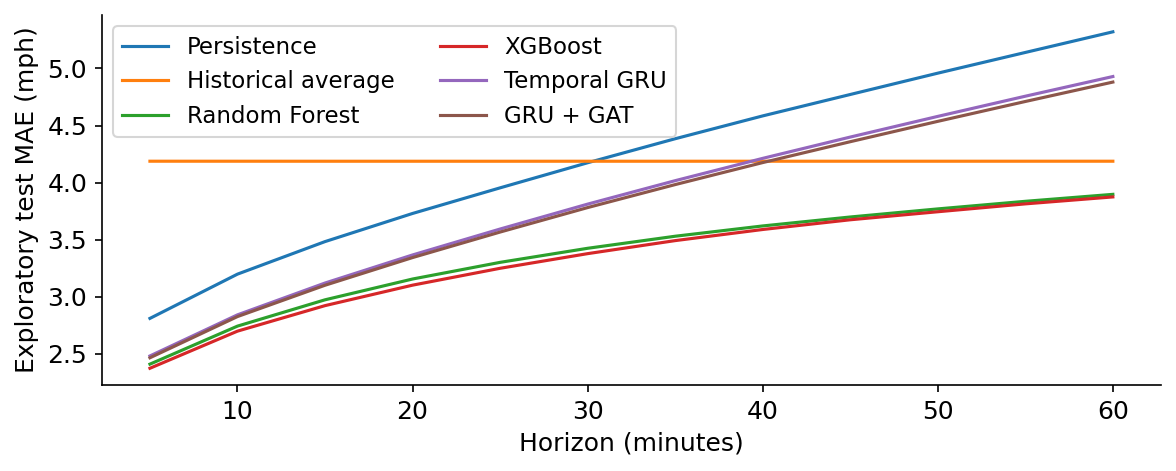
\includegraphics[width=.9\textwidth]{images/horizons.png}\caption{Exploratory test horizon errors; neural curves average seeds.}\end{figure*}

\begin{figure*}[t]\centering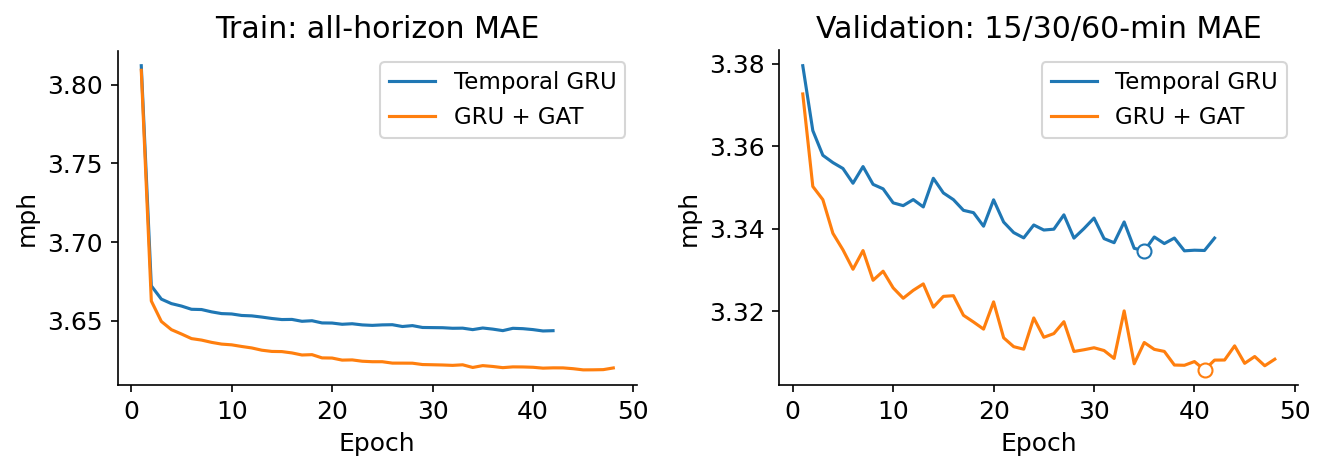
\includegraphics[width=.9\textwidth]{images/learning.png}\caption{Circles mark selected validation epochs. Different horizon aggregations and training/evaluation modes prevent interpreting vertical differences as a matched generalization gap.}\end{figure*}

\begin{figure*}[t]\centering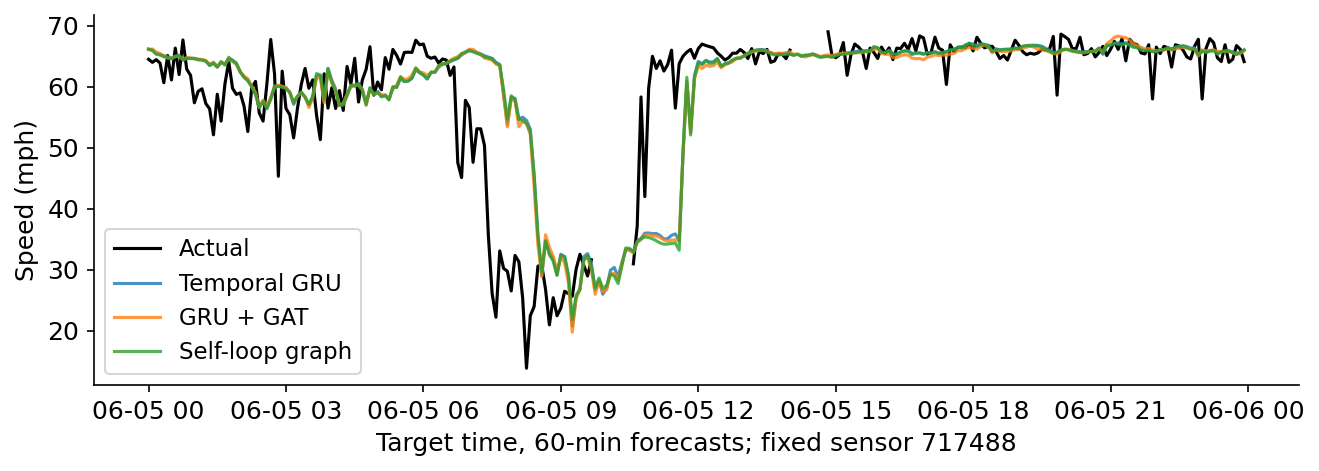
\includegraphics[width=.9\textwidth]{images/forecast.png}\caption{Fixed sensor/day example, not a network-wide performance claim.}\end{figure*}

\begin{figure*}[t]\centering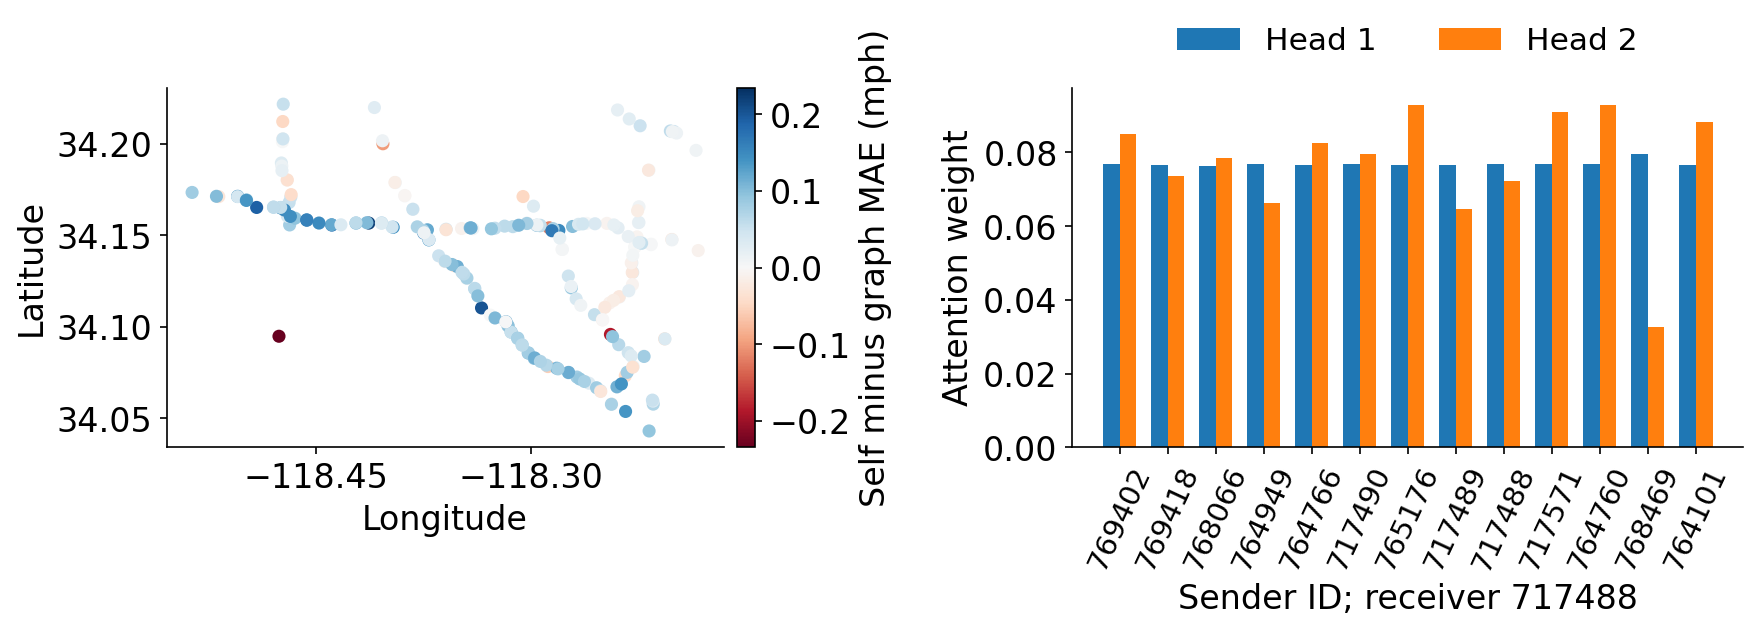
\includegraphics[width=.98\textwidth]{images/spatial_attention.png}\caption{Left: signed seed42 graph improvement, retaining regressions. Right: attention before dropout for a fixed receiver at the first test origin. Weights describe fitted behaviour, not physical causality.}\end{figure*}
}{\textbf{Draft: training/evaluation in progress; no Phase 2 scores yet claimed.}}

\section{Synthetic LWR and Two-Agent Control}
\subsection{Scope and physics}
LWR conserves traffic density $\rho$ and flow $q$:
\[\partial_t\rho+\partial_x q=0,\qquad q=\rho v.\]
Richards motivates macroscopic traffic waves \cite{richards}; the cell-transmission discretization follows the Godunov sending/receiving construction \cite{ctm}. METR-LA lacks measured density, flow and signal actions, so the following experiment is synthetic and separate from the forecasting study. We do not map predicted speeds into invented measured densities.

Six corridor cells lead to one exit. A side cell joins at each of two signalized merges. Agent A controls corridor 1/side 6 into corridor 2; B controls corridor 3/side 7 into corridor 4. Each acts on local approach/downstream occupancy; their actions interact through the corridor. Only one competing movement may have green. All eight cells start empty; three external queues retain arrivals that cannot enter.

Assume $v_f=60$ km/h, backward wave magnitude $w=20$ km/h and jam density $\rho_j=150$ veh/km. These are illustrative, not estimated LA parameters. The triangular diagram gives $Q=v_fw\rho_j/(v_f+w)=2250$ veh/h. For cell density $\rho_i$,
\begin{align}
D_i&=\min(v_f\rho_i,Q),\quad S_i=\min(Q,w(\rho_j-\rho_i)),\\
f_{ij}&=\min(D_i,S_j)\quad\text{on green; zero on red},\\
\rho_i^{k+1}&=\rho_i^k+\frac{\Delta t}{\Delta x}(f_{\rm in}-f_{\rm out}).
\end{align}
Flows are computed from the old state and updated simultaneously. Here $\Delta x=.25$ km and $\Delta t=5$ s satisfy CFL: $\max(v_f,w)\Delta t/\Delta x\leq1$ with hours used in the ratio. Jam storage is 37.5 vehicles/cell. Fractional occupancy represents continuum density.

\subsection{Agents and matched scenarios}
The fixed baseline repeats 40 s main green,5 s clearance,40 s side green,5 s clearance; B has 45 s offset. The responsive agents use pressure proxy $\max(n_{\rm approach}-n_{\rm downstream},0)$, where $n$ is cell vehicle count, including moving traffic. After at least 20 s green, switch when the other pressure is higher by 2 vehicles or the current approach is empty while the other is occupied. Force alternation at 60 s; every switch includes 5 s all-red. This is an occupancy-responsive heuristic inspired by local pressure control \cite{pressure}; we do not transfer its theorem's stability guarantees or claim MARL. The two GAT heads are not these two control agents.

Four predefined scenarios cover balanced, arterial-peak, side-road-peak and downstream-restricted demand. Each has 60 min arrivals plus 20 min drainage, five paired seeds 101--105 and identical arrivals/initial traffic/physics within each policy pair. Fixed signal offsets are part of its declared policy. Parameters, demands and policy rules were recorded before outcomes; no control tuning was performed.

We integrate system occupancy (cells plus external queues) for system vehicle-minutes and external queues for boundary-waiting vehicle-minutes. These are numerical aggregate estimates, not mean completed-trip delay. Throughput and final residuals expose unfinished trips. Forty runs verify conservation, finite state, jam bounds, receiving/sending limits and red gating at every step.
\begin{table*}[t]\centering\small
\caption{Synthetic two-agent comparison: five-seed mean system time and boundary waiting (vehicle-minutes). Equal-green fixed baseline is not demand-optimized. These are not METR-LA or real-world results.}
\begin{tabular}{lrrrr}\toprule
Scenario & Fixed system & Responsive system & Fixed waiting & Responsive waiting\\\midrule
Balanced & 3263.3 & 2212.8 & 1.9 & 1.9\\
Arterial peak & 10850.7 & 2840.5 & 4126.1 & 4.6\\
Side peak & 6435.1 & 3173.6 & 629.4 & 3.3\\
Downstream limit & 14308.9 & 6003.9 & 5720.4 & 334.8\\
\bottomrule\end{tabular}\end{table*}
\begin{table*}[t]\centering\small
\caption{Synthetic mean exit throughput and end-of-horizon residuals, vehicles. Fractional values reflect continuum CTM occupancy, not counted individual cars.}
\begin{tabular}{lrrrr}\toprule
Scenario & Fixed exit & Adapt. exit & Fixed left & Adapt. left\\\midrule
Balanced & 1199.8 & 1199.8 & 0.000 & 0.000\\
Arterial peak & 1450.6 & 1450.6 & 0.011 & 0.000\\
Side peak & 1511.0 & 1511.0 & 0.000 & 0.000\\
Downstream limit & 1516.1 & 1520.2 & 4.058 & 0.000\\
\bottomrule\end{tabular}\end{table*}
\begin{figure*}[t]\centering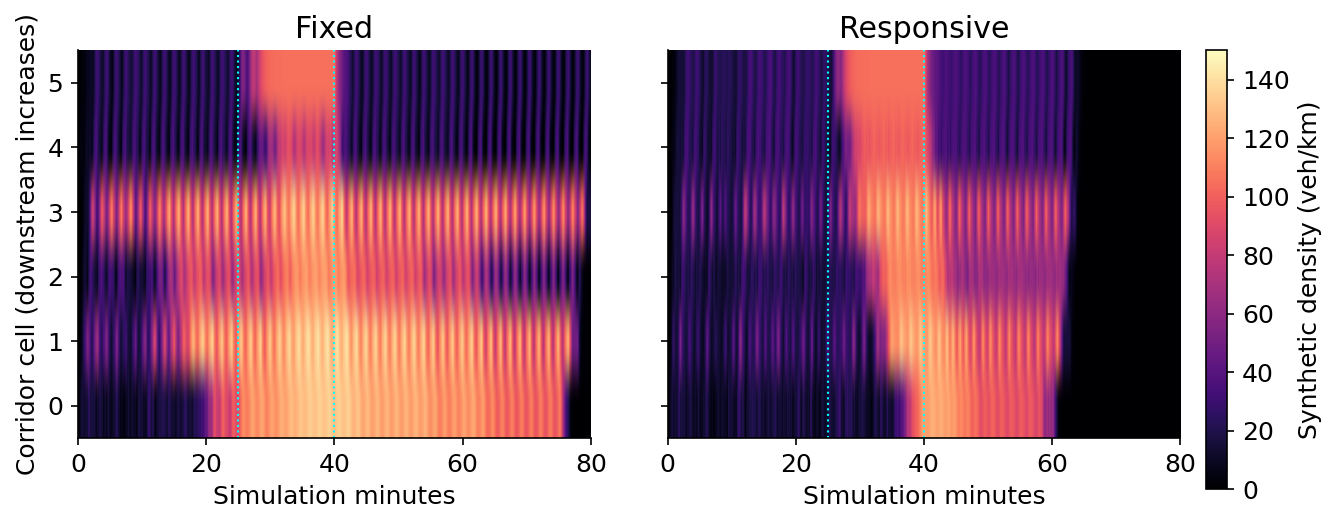
\includegraphics[width=.95\textwidth]{images/control_density.png}
\caption{Synthetic corridor density, downstream-restriction scenario, seed101. Dotted lines bound the reduced exit capacity interval. Density and wave speed are assumed model quantities, not METR-LA measurements.}\end{figure*}


The responsive heuristic lowered system vehicle-time against this equal-green baseline in all four selected scenarios. The baseline is not demand-optimized, so this does not establish optimality or real-city savings. Results do not demonstrate that GAT forecasts improve control. Synthetic parameters, tiny topology, no pedestrian/lane-change model and no calibrated signal dynamics limit transfer. The original faculty technical brief remains unlocated; no particular mandatory simulator or MARL requirement is inferred from the title alone.

\section{Verification and Limitations}
Manifests record source/data/config hashes, normalization, node order and runtime/device. Tests cover causality, fitted statistics, masks, direction, dimensions, gradients and checkpoint/CSV inference. Synthetic overfitting verifies learnability, not traffic performance.
The final local suite passed 76 tests with real data available and no skips (November 16). Lint/format checks passed for 51 Python files. New physics/control tests cover red gating, spillback, CFL, state bounds, conservation, timing and replay. Historical forecast scores and all checkpoint/source identities remain unchanged. No remote CI or native PowerPoint execution is claimed.


The canonical project repository is \url{https://github.com/KatalKavya96/DLML_Midsem_Project}. Run commands and dependency pins are supplied in \texttt{docs/PHASE2\_RUNBOOK.md}. Data, checkpoints and prediction tensors stay local/gitignored; small evidence is retained. The previously exposed test makes results exploratory. Bounded tuning, short history, one region/season, timezone and single-seed auxiliary ablations limit claims. Seed variability is not significance. Negative predictions remain unclipped. Measured results do not certify faculty acceptance or individual understanding.

Host memory pressure prompted a storage-only amendment: construct feature batches on demand rather than retain a 681MB history cache. All 34,249 eligible histories were bitwise equal, fitted statistics were identical and the restarted first epoch reproduced both losses exactly. Five completed fits retain original-source/checkpoint lineage; an unfinished fit restarted from its fixed seed. Model, search, splits and metrics were unchanged. Fit wall times include contention. Incomplete fits restart; optimizer-state continuation is not implemented.

\section{Conclusion}
\IfFileExists{generated/conclusion.tex}{The graph model has mean 60-minute MAE 4.881 mph versus 4.931 mph for its self-loop control and 4.929 mph for the temporal baseline. These comparisons test neighbour access separately from changing model families. Metric and traffic-period trade-offs, seed variability and negative ablations must be retained in interpretation. Among the main rows, XGBoost has the lowest 60-minute MAE and Random Forest the lowest RMSE. Reserved validation selected a pure model, so blending did not earn selection. The exposed evaluation interval remains exploratory; forecasting results do not establish signal-control effectiveness.
}{The study separates temporal learning, graph access and learned weighting. Conclusions must follow measured results, including unsuccessful graph/hybrid experiments. Forecasting does not establish control effectiveness.}

The separate cell-transmission study demonstrates interacting local rule-based signals under declared synthetic assumptions. It does not establish a calibrated end-to-end neural traffic controller.

\section*{Contributions and Assistance}
Kavya Katal coordinates preparation/integration. The extension preserves teammate-prototype and Phase 1 provenance. Phase 2 source, analysis and artifacts use substantial AI assistance. Proposed review scopes: Rudraksh (data/graph), Vridhi (preprocessing/temporal), Anshuman (literature/plots), Bineet (graph/ablations/hybrid), Kavya (integration/evaluation). Assignments do not establish independent implementation; actual member work/understanding requires separate evidence.

\begin{thebibliography}{9}
\bibitem{cho}K. Cho et al., ``Learning Phrase Representations using RNN Encoder--Decoder for Statistical Machine Translation,'' EMNLP, 2014. \url{https://arxiv.org/abs/1406.1078}.
\bibitem{gat}P. Veli\v{c}kovi\'c et al., ``Graph Attention Networks,'' ICLR, 2018. \url{https://arxiv.org/abs/1710.10903}.
\bibitem{dcrnn}Y. Li et al., ``Diffusion Convolutional Recurrent Neural Network: Data-Driven Traffic Forecasting,'' ICLR, 2018. \url{https://arxiv.org/abs/1707.01926}.
\bibitem{richards}P. I. Richards, ``Shock Waves on the Highway,'' Operations Research, 4(1), 42--51, 1956. \url{https://doi.org/10.1287/opre.4.1.42}.
\bibitem{torchgru}PyTorch contributors, ``GRU,'' version 2.7 documentation and installed 2.7.1 module docstring. \url{https://docs.pytorch.org/docs/2.7/generated/torch.nn.GRU.html}.
\bibitem{ctm}A. D. Patire et al., ``Technical Overview of the Cell Transmission Model,'' California PATH, UC Berkeley, July 2015. \url{https://connected-corridors.berkeley.edu/sites/default/files/ctm_technical_overview.pdf}.
\bibitem{pressure}J. Lioris and P. Varaiya, ``Variants of max pressure control for a network of signalized intersections,'' Berkeley research paper. \url{https://connected-corridors.berkeley.edu/sites/default/files/Variants\%20of\%20Max\%20Pressure\%20Control\%20for\%20Signalized\%20Intersections.pdf}.
\end{thebibliography}
\end{document}
